\documentclass[11pt]{article}
\usepackage{graphics,epsfig,amsmath,amssymb}
\usepackage{epsf}
\usepackage{boxedminipage}
\usepackage{fullpage}
\usepackage{fancyheadings}
\usepackage{times}
\usepackage{amsmath}
\usepackage{ifthen}
\usepackage{listings}
%\usepackage{pseudocode}
\usepackage{psfrag}
\usepackage{url}
\pagestyle{fancy}

\setlength{\topmargin}{.2in}
\setlength{\parindent}{0in}
\setlength{\parskip}{.15in}
\setlength{\footskip}{0.1in}

\newcounter{pctr}
\stepcounter{pctr}

\newcounter{partctr}

\newcommand{\ie}{{\em i.e.}}
\newcommand{\eg}{{\em e.g.}}

\newcommand{\ch}{\item {\bf True~~/~~False~~}}
\newcommand{\tfnote}{\probnote{Circle True or False for each choice.}}
\newcommand{\allapply}{\probnote{Circle ALL that apply}}
\newcommand{\bestanswer}{\probnote{Circle the BEST answer}}
\newcommand{\ansbelow}{\probnote{Answer legibly in the space below.}}

\renewcommand{\thesection}{{\bf\Roman{section}}}
\renewcommand{\theenumi}{{\bf\Alph{enumi}.}}
\renewcommand{\labelenumi}{{\bf\Alph{enumi}.}}

\newcommand{\setversion}[1]{\def\version{#1}}
%\setversion{answers}
\setversion{quiz}

\ifthenelse{\equal{\version}{answers}}{
    \newcommand{\sols}[1]{#1}
}{
    \newcommand{\sols}[1]{}
}


\lstdefinelanguage{Pyretic}
{keywords={>>, >+, +, &, push, if_, elif_, else, pop, match, fwd,
    modify, set, mod, drop, $\triangleleft$, announce, withdraw, def}, 
  sensitive=true, alsoletter={-,>>,+,&,|,_},comment=[l][\footnotesize\sffamily\textbf]{\!}
}
\lstset{language=Pyretic,numbers=left}

\begin{document}

\newcounter{answer}
\newenvironment{answer}[1][\relax]{\refstepcounter{answer}\begin{list}%
 {}{\leftmargin 0pt\rightmargin 0pt\labelsep 3pt\parsep 0pt%
 \setlength{\listparindent}{\parindent}}
    \item {\bf Answer \theanswer #1}\
    }{\hspace*{\fill}$\blacksquare$\end{list}} 



% uses these macros to delimit problems
\newcommand\prob[1]%
  {\begin{itemize}\item[]%
   \vspace{.2in}{\bf\thepctr. ~[#1~ points]:}\stepcounter{pctr}}
\newcommand\eprob{\end{itemize}}
\newcommand\probnote[1]%
  {\\\begin{tabular}{cr} \hspace{3in} & {\bf (#1)} \\ \end{tabular}}

% headers/footers
\lhead[\fancyplain{}{\bf Page \thepage ~of \pageref{lastpage}}]%
      {CS 6250 Spring 2014, Quiz 3}
\lfoot[{\bf Name: }]%
      {{\bf Name: }}
\rhead[CS 6250 Spring 2014, Quiz 3]%
      {\fancyplain{}{\bf Page \thepage ~of \pageref{lastpage}}}
\cfoot{}
%\setlength{\headrulewidth}{0in}
\setlength{\headsep}{.3in}

 % Compact itemize and enumerate.  Note that they use the same counters and
% symbols as the usual itemize and enumerate environments.
\def\compactify{\itemsep=0pt \topsep=0pt \partopsep=0pt \parsep=0pt}
\let\latexusecounter=\usecounter
\newenvironment{CompactItemize}
  {\def\usecounter{\compactify\latexusecounter}
   \begin{itemize}}
  {\end{itemize}\let\usecounter=\latexusecounter}
\newenvironment{CompactEnumerate}
  {\def\usecounter{\compactify\latexusecounter}
   \begin{enumerate}}
  {\end{enumerate}\let\usecounter=\latexusecounter}


\cfoot{}
\pagestyle{empty}

\begin{center}
\begin{tabular}{lr}
\resizebox{1in}{!}{\includegraphics{GT}}
&
\parbox{4in}{
    {\Large\it College of Computing} \\ \\
    {\LARGE\sf Georgia Institute of Technology} 
}
%
\end{tabular}
\end{center}

\begin{center}
{\Large{\bf CS 6250: Computer Networking: Spring 2014} \\
 \vspace{.15in} \Huge{\bf Quiz III}} 
%\vspace{.2in}

% this is the box on the first page with overall quiz information
\begin{boxedminipage}[h]{6in}
There are \underline{14 questions} and \underline{\pageref{lastpage}
  pages} in this quiz booklet (including this page).  Answer each
question according to the instructions given.  You have {\bf 85
  minutes}.

%\vspace{.1in} The last page is an easy question.  {\em Rip this
%page off of your exam for five bonus points.}  Turn it in anonymously if
%you like.


\vspace{.1in} 
If you find a question ambiguous, write down any
assumptions you make.  {\bf Be neat and legible.}  If I can't
understand your answer, I can't give you credit!  You may want to look
through the whole quiz to identify which questions you can complete most
quickly for the most points.

\vspace{.1in} 
Use the empty sides of this booklet if you need scratch space.  You
may also use them for answers, although you shouldn't need to.  {\em If you
do use the blank sides for answers, make sure to clearly say so!}

\vspace{.1in} 
{\bf Note well: Write your name in the space below AND your initials at the bottom of each
page of this booklet.}

\begin{center}{\bf THIS IS AN ``CLOSED BOOK'' QUIZ.\\
YOU ARE PERMITTED ONE DOUBLE-SIDED SHEET OF PAPER FOR NOTES.\\
{\em ABSOLUTELY NO EMAIL OR MESSAGING OF ANY KIND!} \\
MAKE SURE YOU'VE READ ALL THE INSTRUCTIONS ABOVE!}
\end{center}
{\em Initial here to indicate that (1)~you've read the instructions and (2)~
you agree to abide by the Georgia Tech Honor Code: }

%\vspace{.1in} The last page has easy bonus questions, which you can
%answer outside of the allotted time.  Rip the last page off of your
%quiz for five bonus points.  Turn it in anonymously if you like.

\end{boxedminipage}
\end{center}
\vspace*{0.25in}
\begin{center}
{\it Do not write in the boxes below}
\end{center}

\begin{center}
\begin{tabular}{|l|l|l|l|l|l|l|l|l|} \hline \hline
{\bf 1-5 (xx/20)}& {\bf 6-9 (xx/20)}& {\bf 10-12 (xx/40)} & {\bf 13-14 (xx/20)} & {\bf Total
  (xx/100)}  \\ \hline 
 & & & & \\ 
 & & & &\\ \hline \hline
\end{tabular}
\end{center}

\vspace{.2in}
{\bf\Large{Name:}}

\newpage
\pagestyle{fancy}

\section{Warmup}

\prob{4} What are some advantages of separating the data and control
planes, as in a software defined network (SDN)?
\allapply

\setcounter{partctr}{0}
\begin{list}{\bf\Alph{partctr}.}{\usecounter{partctr}}
\item Independent evolution of data and control plane.
\item Less likelihood of failure.
\item Network-wide view of the state of forwarding elements.
\item Ability to control a network from a single, centralized software program.
\item None of the above.
\end{list}
\eprob

\sols{
\begin{answer}
\end{answer}
}


\prob{4} What is the meaning of ``parallel composition'', in terms of
Pyretic policies?
\allapply
\setcounter{partctr}{0}
\begin{list}{\bf\Alph{partctr}.}{\usecounter{partctr}}
%\begin{enumerate}
\item Apply each policy to the same copy of the packet concurrently.
\item Apply multiple policies to packets in sequence.
\item Make a copy of the original packet, then apply each policy to an
  independent copy of the packet.
\item Apply exactly one of the parallel policies to a copy of the
  packet, depending on which policy matches.
\item All of the above.
\end{list}
\eprob

\sols{
\begin{answer}
\end{answer}
}

\prob{4} What does the Pyretic policy {\tt match(srcip=A) >> fwd(2)} do?
\allapply
\setcounter{partctr}{0}
\begin{list}{\bf\Alph{partctr}.}{\usecounter{partctr}}
%\begin{enumerate}
\item For all packets that will be forwarded via output port 2, rewrite
the source IP address to A.
\item Forward packets matching source IP address A via output port 2.
\item Rewrite packets matching source IP address A so that the virtual packet
  header for {\tt outport} has the value 2.
\item Drop packets whose source IP address is not A.
\item All of the above
\end{list}
\eprob

\sols{
\begin{answer}
\end{answer}
}

%% \newpage
%% \prob{4} 
%% What are some mechanisms to create virtual hosts and links in a virtual network?
%% \allapply
%% \setcounter{partctr}{0}
%% \begin{list}{\bf\Alph{partctr}.}{\usecounter{partctr}}
%% %\begin{enumerate}
%% \item Virtual links with IP-in-IP tunnels
%% \item Virtual links with Ethernet-in-IP (EGRE) encapsulation
%% \item Virtual hosts with virtual machines
%% \item Virtual hosts with virtual environments
%% \item All of the above
%% \end{list}
%% \eprob

%% \sols{
%% \begin{answer}
%% \end{answer}
%% }


\newpage
\prob{4}  Which of the following are true about BGP routing security?
\allapply
\setcounter{partctr}{0}
\begin{list}{\bf\Alph{partctr}.}{\usecounter{partctr}}
%\begin{enumerate}
\item An AS can defend against route hijack attacks by filtering route
  advertisements for IP prefixes that neighbors do not own.
\item An AS can defend against AS path shortening attacks by filtering
  route advertisements for AS paths that it does not own.
\item In Secure BGP (S-BGP), an AS that advertises a route signs a
  version of the AS path that includes the next AS along the path (i.e.,
  the AS to whom it is advertising the route).
\item Attackers can use short-lived BGP routing announcements to make it
  more difficult to trace certain types of attacks (e.g., spam, DoS).
\item None of the above
\end{list}
\eprob

\sols{
\begin{answer}
\end{answer}
}

\prob{4}  What are some mechanisms that can be used to implement censorship?
\allapply
\setcounter{partctr}{0}
\begin{list}{\bf\Alph{partctr}.}{\usecounter{partctr}}
%\begin{enumerate}
\item Blocking DNS requests.
\item Blocking TCP connections.
\item Redirecting URLs to a block page.
\item Withdrawing BGP routes.
\item None of the above.
\end{list}
\eprob

\sols{
\begin{answer}
\end{answer}
}





\newpage
\section{Potpourri}

\prob{5} Define {\em origin authentication} and {\em path
  authentication}, in the context of interdomain routing security.
Describe an attack that is possible without origin authentication, and
describe an attack that is possible without path authentication.
~\ansbelow
\vspace*{2.5in}
\eprob


\prob{5} Mininet uses virtual ``containers'' to create each virtual node
in an emulated virtual network.  Explain the difference between a
virtual container and a virtual machine, and describe one advantage of
using virtual containers over virtual machines for network emulation (as
in Mininet).  ~\ansbelow
\vspace*{1.5in}
\eprob

\newpage
\prob{5} One problem that software defined networks face is that of
{\em consistent updates}.  Define per-packet consistency and per-flow
consistency.  Give an example of incorrect behavior that can result if
the network does not provide per-packet consistency, and an example of
incorrect behavior that can result if the network does not provide
per-flow consistency. ~\ansbelow
\vspace*{2.5in}
\eprob

\prob{5} Explain what equal cost multipath (ECMP) is, and how it can be
used in a data center to balance load across servers in a data center.
(You may wish to draw a picture of a standard data center topology an
explain where ECMP can be used to balance load across certain links.)~\ansbelow
\vspace*{1.5in}
\eprob



\newpage
\section{Programming SDNs}

\prob{20} 
In this problem, you will explore a few simple programs in Pyretic and
PyResonance, applying what you learned in the lecture videos and problem
sets.  Consider the code sample below from the Pyretic examples, which performs simple MAC
learning: 

\begin{scriptsize}
\begin{lstlisting}
def learn(self):

    def update_policy():
        self.policy = self.forward + self.query
    self.update_policy = update_policy

    def learn_new_MAC(pkt):
        self.forward = if_(match(dstmac=pkt['srcmac'],
                                switch=pkt['switch']),
                          fwd(pkt['inport']),
                          self.forward) 
        self.update_policy()

    def set_initial_state():
        self.query = packets(1,['srcmac','switch'])
        self.query.register_callback(learn_new_MAC)
        self.forward = self.flood  
        self.update_policy()

    self.flood = flood()           
    set_initial_state()


def mac_learner():
    return dynamic(learn)()

def main():
    return mac_learner()
\end{lstlisting}
\end{scriptsize}


\begin{enumerate}
\item Explain the meaning of the {\tt packets} statement (line 15).
\item Explain what line 4 does.
\item Explain why the {\tt match} statement on lines 8--9 matches on a
  the {\tt switch} field.
\item According to line 17, the initial {\tt self.forward} policy is
  {\tt flood()}.  Upon the first callback to {\tt learn\_new\_MAC}, {\tt
    self.forward} is reassigned.  
  \begin{itemize}
    \item Explain when this callback takes place.
    \item Suppose that a packet with source MAC
      address {\tt ab:cd:ef:ab:cd:ef} arrives on input port {\tt 1} on
      switch {\tt A}.  Write the forwarding policy in terms of {\tt match},
      {\tt fwd}, and {\tt flood}, and explain how new packet arrivals cause
      the program to ``learn'' new forwarding behavior.
  \end{itemize}
\end{enumerate}


~\ansbelow\probnote{You can use the back of the page as well.}
\vspace{2in}
\eprob

\sols{
\vspace{-1in}
\begin{answer}
% http://blog.thousandeyes.com/a-very-simple-model-for-tcp-throughput/
\end{answer}
}

\newpage
\prob{10} George Burdell wants to modify the learning switch to create a
firewall, as you have done in the assignments.  He adds the following
functions:

\begin{scriptsize}
\begin{lstlisting}
def firewall(self):

  def update_policy():
    self.policy = self.policy + self.query
  self.update_policy = update_policy

  def initialize():

    self.AddRule(1,'00:00:00:00:00:01')
    self.AddRule(1,'00:00:00:00:00:02')
    
    self.query = packets(None, ['srcmac'])
    self.query.register_callback(check_rules)

    self.policy = drop
    self.update_policy()

  def check_rules(pkt):
    filter_on_mac(pkt)

  def filter_on_mac(pkt):
    if self.CheckRule(pkt['switch'], pkt['srcmac']) == True:
        self.policy = passthrough
    else:
        self.policy = drop
    self.update_policy()

  initialize()

def main():
    return dynamic(firewall)() >> dynamic(learn)()
\end{lstlisting}
\end{scriptsize}
Assume that {\tt AddRule} adds a rule to firewall with ID {\tt 1} that
permits packets with the source MAC address provided, that {\tt
  CheckRule} checks for the presence of a permit rule at a switch for
frames with the corresponding source MAC address, and that {\tt learn}
implements a simple MAC learner.

\begin{enumerate}
\item George starts his control program and begins to send pings between
  host 1 and host 2.  The firewall passes traffic between these two
  hosts just fine.  However, when he sends pings between host 1 and host
  3, he notices that some traffic actually passes between these two
  hosts, even though there is no rule in the table for the host with MAC
  address 3.  Why?  
\item Briefly explain how you would fix the problem that George
  observes.  (You don't have to write any code to receive credit, although you are welcome to
  if it makes your answer more clear.)
\end{enumerate}

 
~\ansbelow\probnote{You can use the back of the page as well.}
\vspace{2in}
\eprob


\prob{10} In a common SDN control program, if a packet arrives at the
switch and the switch has no matching flow table entry for the packet,
the switch must send the packet to the controller.
\begin{itemize}
\item Explain why sending data packets to the controller is not
  desirable.
\item With advance knowledge of traffic
  patterns, it might be possible to avoid sending traffic to the
  controller.  Describe a mechanism for handling as much
  traffic as possible in the data path.  Mention possible scalability
  concerns with your approach, and possible ways to address them.
\end{itemize}
~\ansbelow
\vspace{2in}
\eprob

\sols{
\vspace{-1in}
\begin{answer}
% http://blog.thousandeyes.com/a-very-simple-model-for-tcp-throughput/
\end{answer}
}



\newpage
\section{Censorship}

\prob{10} 
Consider the figure below, which shows a Tor network, including a guard
node, a relay node, and an exit node.  

\centering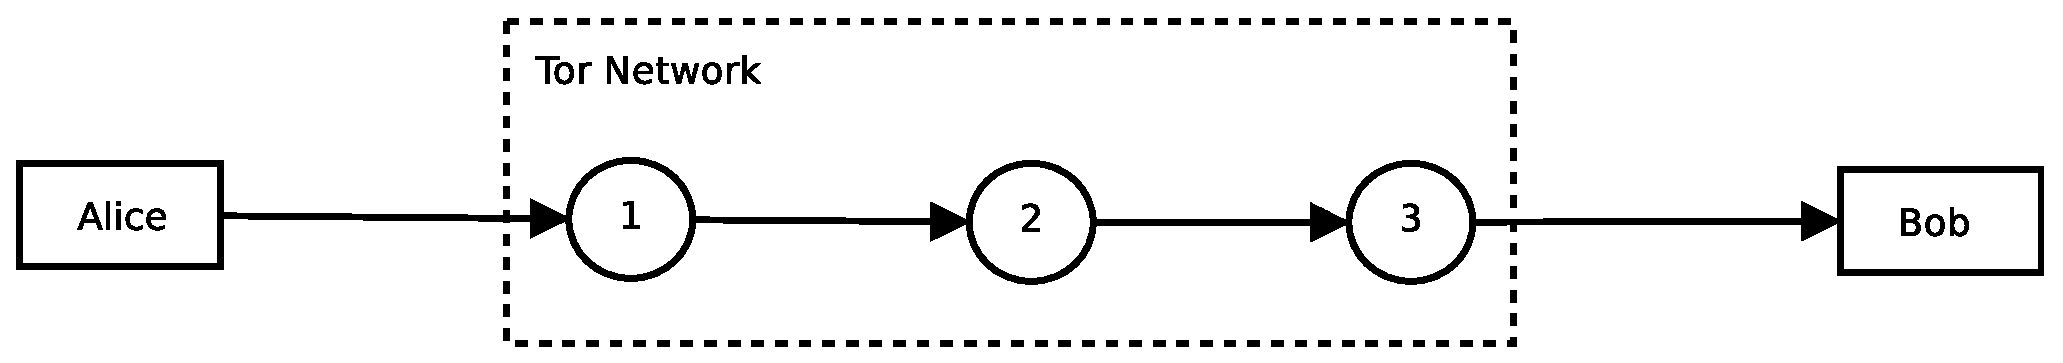
\includegraphics[width=0.95\linewidth]{tor}

\begin{enumerate}
\item Which of the links in the diagram are encrypted? 
\item Above each link in the diagram, write down the onion encryption for a
  Tor packet as it traverses the path from Alice to Bob, using the
  notation $\{M\}_{k_1}$ to indicate that the message $M$ is encrypted
  with the public key of node $1$.  You can (and should) use nested
  encryption.  
\item Explain how this mode of onion encryption makes it impossible for
  an intermediate relay in the Tor network to know either the sender or
  recipient of traffic.
\item Suppose that an attacker could observe traffic both entering and
  exiting the Tor network.  What types of attacks could an attacker
  mount, in this case?
\end{enumerate}

~\ansbelow
\vspace{2in}
\eprob

\newpage
\prob{10} 
George Burdell notes that, with knowledge of the Tor relays, a censor
could simply add firewall rules to block traffic to all of the IP
addresses of Tor relays.   Explain how you might design a client lookup service such that no
  single client can discover all Tor relay nodes.  
~\ansbelow
\vspace{2in}
\eprob



\label{lastpage}
\end{document}
